%
% entwicklungssatz.tex
%
% (c) 2018 Prof Dr Andreas Müller, Hochschule Rapperswil
%
\section{Entwicklungssatz\label{entwicklungssatz}}
\rhead{Entwicklungssatz}
\index{Entwicklungssatz}
\index{rekursiv}
Der Entwicklungssatz erlaubt, Determinanten rekursiv zu berechnen.
Für die Berechnung einer $n\times n$-Determinante werden $n$
$(n-1)\times(n-1)$-Determinanten bestimmt und miteinander verknüpft.
Die Entwicklung einer Determinante erfolgt einer Spalte oder Zeile.
Da wir durch Vertauschungen und Transposition diese Zeile oder Spalte
immer zur vordersten Spalte machen können, stellen wir nur die
Entwicklung der Determinante nach der ersten Spalte dar.

%
% entwicklungssatz.tex -- neue version der Darstelllung des Entwicklungssatzes
%
% (c) 2017 Prof Dr Andreas Müller, Hochschule Rapperswil
%
\subsection{Entwicklungssatz aus der Pivotproduktformel}
Die Pivotproduktformel erlaubt, die Determinante einer Dreiecksmatrix sofort
zu berechnen:
\[
\left|\begin{matrix}
a_{11}&a_{12}&a_{13}&\dots &a_{1n}\\
  0   &a_{22}&a_{23}&\dots &a_{2n}\\
  0   &  0   &a_{33}&\dots &a_{3n}\\
\vdots&\vdots&\vdots&\ddots&\vdots\\
  0   &  0   &   0  &  0   &a_{nn}
\end{matrix}\right|
=
a_{11}\cdot a_{22}\cdot a_{33}\cdot\dots\cdot a_{nn}.
\]
Es lässt sich daraus aber eine viel allgemeinere Beobachtung ableiten, die
schliesslich zu einer allgemeinen Berechnungsformel für die Determinante
führt, dem Entwicklungssatz.

\subsubsection{Rekursion}
Wir betrachten die Determinante, die in der ersten Spalte nur in der
ersten Zeile ein von Null verschiedenes Element enthält:
\[
%\left|\begin{matrix}
A=
\begin{pmatrix}
a_{11}&a_{12}&a_{13}&\dots &a_{1n}\\
  0   &a_{22}&a_{23}&\dots &a_{2n}\\
  0   &a_{32}&a_{33}&\dots &a_{3n}\\
\vdots&\vdots&\vdots&\ddots&\vdots\\
  0   &a_{n2}&a_{n3}&\dots &a_{nn}
\end{pmatrix}.
%\end{matrix}\right|
\]
Nach der Pivotproduktformel ist $a_{11}$ das erste Pivot-Element.
Es muss jetzt nur noch der Gaussalgorithmus in der verbleibenden Matrix
\[
A_{11}
=
\begin{pmatrix}
a_{22}&a_{23}&\dots &a_{2n}\\
a_{32}&a_{33}&\dots &a_{3n}\\
\vdots&\vdots&\ddots&\vdots\\
a_{n2}&a_{n3}&\dots &a_{nn}
\end{pmatrix}
\]
bestimmt werden.
Die weggelassene erste Zeile und Spalte hat keinen Einfluss darauf, wie
der Gauss-Algorithmus in $A_{11}$ durchgeführt wird.
Die Pivotproduktformel liefert daher die Rekursionsformel
\begin{equation}
\det(A)
=
a_{11}\cdot
\left|\begin{matrix}
a_{22}&a_{23}&\dots &a_{2n}\\
a_{32}&a_{33}&\dots &a_{3n}\\
\vdots&\vdots&\ddots&\vdots\\
a_{n2}&a_{n3}&\dots &a_{nn}
\end{matrix} \right|
=
a_{11}
\det(A_{11}).
\label{determinante:entwicklungssatz:rekursion}
\end{equation}

\subsubsection{Vorzeichenregel}
Die Rekursionsformel~\eqref{determinante:entwicklungssatz:rekursion}
kann verallgemeinert werden auf eine Situation, wo in Spalte $k$
nur ein Element, nämlich das in Zeile $i$, von Null verschieden ist.
\[
A=
\begin{pmatrix}
a_{  1 1}&\dots &a_{  1,k-1}&a_{  1 k}&a_{  1,k+1}&\dots &a_{  1 n}\\
\vdots   &\ddots&\vdots     &\vdots   &\vdots     &\ddots&\vdots   \\
a_{i-1,1}&\dots &a_{i-1,k-1}&a_{i-1,k}&a_{i-1,k+1}&\dots &a_{i-1,n}\\
a_{  i 1}&\dots &a_{  i,k-1}&a_{  i k}&a_{  i,k+1}&\dots &a_{  i n}\\
a_{i+1,1}&\dots &a_{i+1,k-1}&a_{i+1,k}&a_{i+1,k+1}&\dots &a_{i+1,n}\\
\vdots   &\ddots&\vdots     &\vdots   &\vdots     &\ddots&\vdots   \\
a_{  n 1}&\dots &a_{  n,k-1}&a_{  n k}&a_{  n,k+1}&\dots &a_{  n n}
\end{pmatrix}
\]
Durch Vertauschung mit den $i-1$ vorangegangenen Zeilen und $k-1$
vorangegangen Spalten kann man erreichen, dass das Element $a_{ik}$
in die linke obere Ecke verschoben wird.
Bei den Zeilenvertauschungen ändert das Vorzeichen $(i-1)$-mal, also
um $(-1)^{i-1}$, bei den Spaltenvertauschungen um den Faktor $(-1)^{k-1}$.
Insgesamt erhalten wir daher die Formel
\begin{align*}
\det(A)
&=
(-1)^{i-1}(-1)^{k-1}
\left|\;\begin{matrix}
a_{ik}&a_{  i 1}&\dots &a_{  i,k-1}&a_{  i,k+1}&\dots &a_{  i n}\\
  0   &a_{  1 1}&\dots &a_{  1,k-1}&a_{  1,k+1}&\dots &a_{  1 n}\\
\vdots&\vdots   &\ddots&\vdots     &\vdots     &\ddots&\vdots   \\
  0   &a_{i-i,1}&\dots &a_{i-i,k-1}&a_{i-1,k+1}&\dots &a_{i-i,n}\\
  0   &a_{i+i,1}&\dots &a_{i+i,k-1}&a_{i+1,k+1}&\dots &a_{i+i,n}\\
\vdots&\vdots   &\ddots&\vdots     &\vdots     &\ddots&\vdots   \\
  0   &a_{  n 1}&\dots &a_{  n,k-1}&a_{  n,k+1}&\dots &a_{  n n}
\end{matrix}\;\right|
\\
&=
(-1)^{i+k-2}
\cdot
a_{ik}
\cdot
\left|\;\begin{matrix}
a_{  1 1}&\dots &a_{  1,k-1}&a_{  1,k+1}&\dots &a_{  1 n}\\
\vdots   &\ddots&\vdots     &\vdots     &\ddots&\vdots   \\
a_{i-i,1}&\dots &a_{i-i,k-1}&a_{i-1,k+1}&\dots &a_{i-i,n}\\
a_{i+i,1}&\dots &a_{i+i,k-1}&a_{i+1,k+1}&\dots &a_{i+i,n}\\
\vdots   &\ddots&\vdots     &\vdots     &\ddots&\vdots   \\
a_{  n 1}&\dots &a_{  n,k-1}&a_{  n,k+1}&\dots &a_{  n n}
\end{matrix}\;\right|
=
(-1)^{i+k}\det(A_{ik}),
\end{align*}
darin haben wir mit $A_{ik}$ die Matrix abgekürzt, die aus $A$ durch
Weglassen der Zeile $i$ und der Spalte $k$ entsteht.
Das Vorzeichen $(-1)^{i+k}$ kann dem folgenden Schachbrettmuster
entnommen werden:
\begin{center}
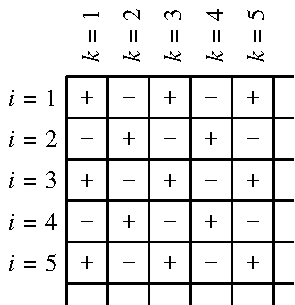
\includegraphics{2/images/schachbrett.pdf}
\end{center}

\subsubsection{Aufteilung einer Spalte}
Enthält eine Spalte nur ein einziges von Null verschiedenes Element,
können wir die Determinante auf die Berechnung einer kleineren
Determinante reduzieren.
Um dies für die Berechnung einer beliebigen Determinante ausnützen
zu können, müssen wir in der Lage sein, eine beliebige Spalte in Spalten
aufzuteilen, die nur ein einziges von Null verschiedenes Element
enthalten.
Dies gelingt mit Hilfe der Linearität.

Wir zeigen das Prinzip am Beispiel der ersten Spalte.
Die Linearität liefert
\begin{align}
\left|\begin{array}{cccc}
a_{11}&a_{12}&\dots &a_{1n}\\
a_{21}&a_{22}&\dots &a_{2n}\\
a_{31}&a_{32}&\dots &a_{3n}\\
\vdots&\ddots&\ddots&\vdots\\
a_{n1}&a_{n2}&\dots &a_{nn}\\
\end{array}\right|
&=
\left|\begin{array}{c@{\hskip2pt}c@{\hskip2pt}cccc}
a_{11}&+&  0   &a_{12}&\dots &a_{1n}\\
  0   &+&a_{21}&a_{22}&\dots &a_{2n}\\
  0   &+&a_{31}&a_{32}&\dots &a_{3n}\\
\vdots& &\vdots&\ddots&\ddots&\vdots\\
  0   &+&a_{n1}&a_{n2}&\dots &a_{nn}\\
\end{array}\right|
\notag
\\
&=
\left|\begin{array}{cccc}
a_{11}&a_{12}&\dots &a_{1n}\\
  0   &a_{22}&\dots &a_{2n}\\
  0   &a_{32}&\dots &a_{3n}\\
\vdots&\ddots&\ddots&\vdots\\
  0   &a_{n2}&\dots &a_{nn}\\
\end{array}\right|
+
\left|\begin{array}{cccc}
  0   &a_{12}&\dots &a_{1n}\\
a_{21}&a_{22}&\dots &a_{2n}\\
a_{31}&a_{32}&\dots &a_{3n}\\
\vdots&\ddots&\ddots&\vdots\\
a_{n1}&a_{n2}&\dots &a_{nn}\\
\end{array}\right|.
\label{determinate:entwicklungssatz:aufspaltung}
\end{align}
Durch wiederholte Anwendung dieser Idee kann die erste Spalte in $n$
Spalten aufgeteilt werden, die jede nur ein einziges von Null verschiedenes
Element enthält.

\subsubsection{Allgemeiner Fall}
Damit haben wir alle Komponenten für die allgemeine Berechnungsformel
zusammen.
Wir wählen dazu die Spalte $k$ aus.
Die Aufspaltungsformel
\eqref{determinate:entwicklungssatz:aufspaltung}
besagt, dass wir eine Determinante zerlegen können in eine Summe von
speziellen Determinanten, in denen die Spalte $k$ jeweils nur ein
von Null verschiedenes Elemente enthält.
Diese Elemente sind die Spaltenelemente $a_{ik}$ mit $1\le i\le n$.

Die Rekursionsformel \eqref{determinante:entwicklungssatz:rekursion}
besagt, dass wir diese Determinanten berechnen können aus der
Determinante der Matrix, in der man die Zeile $i$ und die Spalte $k$
weggelassen hat.
Die Vorzeichenregel sagt, welches Vorzeichen man dazu verwenden muss.
Insgesamt bekommen wir so die Formel
\[
\det(A)
=
\sum_{i=1}^n
\underbrace{ (-1)^{i+k}}_{\text{Vorzeichen }}
\underbrace{
a_{ik}
\cdot
\det(A_{ik}).
}_{\text{Rekursion nach 
\eqref{determinante:entwicklungssatz:rekursion}}}
\]
Sie heisst der {\em Entwicklungssatz}.
\index{Entwicklungssatz}




\subsection{Entwicklungssatz direkt aus der Linearität}
Man kann den Entwicklungssatz auch ganz direkt aus der Linearität
und den Rechenregeln für die Determinante einer Matrix $A$ herleiten.
Seien also $a_{ij}$ die Einträge in einer $n\times n$-Determinante.
Die erste Spalte können wir als Summe von Vektoren betrachten,
die jeweils nur an einer Stelle eine Eins haben und sonst aus
Nullen bestehen:
\[
\begin{pmatrix}
a_{11}\\a_{21}\\\vdots\\a_{n1}
\end{pmatrix}
=
a_{11}\begin{pmatrix}1\\0\\\vdots\\0\end{pmatrix}
+
a_{21}\begin{pmatrix}0\\1\\\vdots\\0\end{pmatrix}
+
\dots
+
a_{n1}\begin{pmatrix}0\\0\\\vdots\\1\end{pmatrix}
\]
Da die Determinante eine lineare Funktion der Spalten ist,
können wir dies einsetzen:
\begin{align*}
\det(A)
%=
%\left|\;
%\begin{matrix}
%a_{11}&a_{12}&\dots&a_{1n}\\
%a_{21}&a_{22}&\dots&a_{2n}\\
%\vdots&\vdots&\ddots&\vdots\\
%a_{n1}&a_{n2}&\dots&a_{nn}
%\end{matrix}
%\;\right|
&=
a_{11}
\left|\;
\begin{matrix}
1&a_{12}&\dots&a_{1n}\\
0&a_{22}&\dots&a_{2n}\\
\vdots&\vdots&\ddots&\vdots\\
0&a_{n2}&\dots&a_{nn}
\end{matrix}
\;\right|
+a_{21}
\left|\;
\begin{matrix}
0&a_{12}&\dots&a_{1n}\\
1&a_{22}&\dots&a_{2n}\\
\vdots&\vdots&\ddots&\vdots\\
0&a_{n2}&\dots&a_{nn}
\end{matrix}
\;\right|
+\dots
\\
&\qquad
+a_{n1}
\left|\;
\begin{matrix}
0&a_{12}&\dots&a_{1n}\\
0&a_{22}&\dots&a_{2n}\\
\vdots&\vdots&\ddots&\vdots\\
1&a_{n2}&\dots&a_{nn}
\end{matrix}
\;\right|
\end{align*}
Durch Vertauschungen kann man die Zeile, die mit $1$ beginnt, in jeder
Determinante nach oben bringen, die einzelnen Terme erhalten dadurch
alternierende Vorzeichen
\begin{align*}
\det(A)
&=
a_{11}
\left|\;
\begin{matrix}
1&a_{12}&\dots&a_{1n}\\
0&a_{22}&\dots&a_{2n}\\
\vdots&\vdots&\ddots&\vdots\\
0&a_{n2}&\dots&a_{nn}
\end{matrix}
\;\right|
-a_{21}
\left|\;
\begin{matrix}
1&a_{22}&\dots&a_{2n}\\
0&a_{12}&\dots&a_{1n}\\
\vdots&\vdots&\ddots&\vdots\\
0&a_{n2}&\dots&a_{nn}
\end{matrix}
\;\right|
+\dots
\\
&\qquad
+(-1)^{n+1}a_{n1}
\left|\;
\begin{matrix}
1&a_{n2}&\dots&a_{nn}\\
0&a_{12}&\dots&a_{1n}\\
0&a_{22}&\dots&a_{2n}\\
\vdots&\vdots&\ddots&\vdots\\
0&a_{n-1,2}&\dots&a_{n-1,n}
\end{matrix}
\;\right|
\end{align*}
Um die einzelnen Determinanten zu berechnen, muss man jetzt 
den Gauss-Algorithmus anwenden.
In der ersten Zeile und Spalte
gibt es nichts mehr zu tun, das dort stehende Pivot-Element ist
bereits $1$.
Es bleibt also nur noch die $(n-1)\times(n-1)$-Matrix
im rechten unteren Teil, diese besteht aus den Zeilen und Spalten
von $A$ die übrig bleiben, wenn man die erste Spalte wegstreicht,
und im $i$-ten Summanden die $i$-te Zeile.
Der Gauss-Algorithmus wird
die Determinante dieser $(n-1)\times(n-1)$ Matrix liefern.
\begin{align*}
\det(A)
&=
a_{11}
\left|\;
\begin{matrix}
a_{22}&\dots&a_{2n}\\
a_{32}&\dots&a_{3n}\\
\vdots&\ddots&\vdots\\
a_{n2}&\dots&a_{nn}
\end{matrix}
\;\right|
-a_{21}
\left|\;
\begin{matrix}
a_{12}&\dots&a_{1n}\\
a_{32}&\dots&a_{3n}\\
\vdots&\ddots&\vdots\\
a_{n2}&\dots&a_{nn}
\end{matrix}
\;\right|
+\dots
\\
&\qquad
+(-1)^{n+1}a_{n1}
\left|\;
\begin{matrix}
a_{12}&\dots&a_{1n}\\
a_{22}&\dots&a_{2n}\\
\vdots&\ddots&\vdots\\
a_{n-1,2}&\dots&a_{n-1,n}
\end{matrix}
\;\right|
\end{align*}
Wir verwenden folgende Notation, um diese Formel noch etwas kompakter
auszudrücken.
\index{Minor}
\begin{definition}Sei $A$ eine $n\times n$-Matrix mit Einträgen $a_{ij}$.
Dann heisst die Matrix $A_{ij}$, die sich aus $A$ durch wegstreichen
der $i$-ten Zeile und der $j$-ten Spalte ergibt, der $i$-$j$-Minor der
Matrix $A$.
\end{definition}
Damit kann der Determinantenentwicklungssatz nun wie folgt formuliert
werden:
\begin{satz}
Sei $A$ eine $n\times n$-Matrix.
Dann ist
\[
\det(A)=
\sum_{i=1}^n(-1)^{i+1}a_{i1}\det(A_{i1})
=
\sum_{i=1}^n(-1)^{1+j}a_{1j}\det(A_{1j})
\]
die Entwicklung nach der ersten Spalte bzw.~Zeile, und 
\[
\det(A)=
\sum_{i=1}^n(-1)^{i+j}a_{ij}\det(A_{ij})
=
\sum_{j=1}^n(-1)^{i+j}a_{ij}\det(A_{ij})
\]
die Entwicklung nach der $j$-ten Spalte bzw.~$i$-ten Zeile. 
\end{satz}

\begin{beispiel}Die zu Beginn des Kapitels gefundene Formel für
die Determinante einer $2\times 2$-Matrix ist ein Spezialfall
des Entwicklungssatzes
\[
\left|\;
\begin{matrix}
a&b\\c&d
\end{matrix}
\;\right|
=a\cdot\det(d)-b\cdot\det(c)=ad-bc.
\]
\end{beispiel}

\begin{beispiel}
Man berechne die Determinante der Matrix
\[
A=\begin{pmatrix}
-1&-3&0\\
2&3&-2\\
2&1&-3
\end{pmatrix}
\]
Der Entwicklungssatz liefert
\begin{align*}
\det(A)&=
-1\det\begin{pmatrix}3&-2\\1&-3\end{pmatrix}
-2\det\begin{pmatrix}-3&0\\1&-3\end{pmatrix}
+2\det\begin{pmatrix}-3&0\\3&-2\end{pmatrix}
\\
&=
-1(-9+2)-2(9-0)+2(6-0)=7-18+12=1.
\end{align*}
\end{beispiel}

\subsection{Spezialfall: Dimension 3, die Sarrus Formel}
\index{Sarrus-Formel}
Mit diesem Satz lässt sich jetzt auch die Sarrussche Formel einfach beweisen:
\begin{align*}
\left|\;
\begin{matrix}
a_{11}&a_{12}&a_{13}\\
a_{21}&a_{22}&a_{23}\\
a_{31}&a_{32}&a_{33}
\end{matrix}\;\right|
&=
a_{11}
\left|\;\begin{matrix}
a_{22}&a_{23}\\
a_{32}&a_{33}
\end{matrix}\;\right|
-
a_{21}
\left|\;\begin{matrix}
a_{12}&a_{13}\\
a_{32}&a_{33}
\end{matrix}\;\right|
+
a_{31}
\left|\;\begin{matrix}
a_{12}&a_{13}\\
a_{22}&a_{23}
\end{matrix}\;\right|
\\
&=a_{11}(a_{22}a_{33}-a_{23}a_{32})
-a_{21}(a_{12}a_{33}-a_{13}a_{32})
+a_{31}(a_{12}a_{23}-a_{13}a_{22})
\\
&=
a_{11}a_{22}a_{33}+a_{12}a_{23}a_{31}+a_{13}a_{21}a_{32}
-a_{31}a_{22}a_{13}-a_{32}a_{23}a_{11}-a_{33}a_{21}a_{12}
\end{align*}
Achtung: diese Formel kann nicht auf grössere Determinanten
verallgemeinert werden.

